\PassOptionsToPackage{dvipsnames}{xcolor}
\documentclass[a4paper,11pt]{report} %article

\usepackage{graphicx,subfigure,afterpage,hyperref,xspace,xcolor,caption,soul,geometry,pdfpages,stackengine,eso-pic,fancyhdr,hyphenat,listings,longtable,url,enumitem,fancyvrb}


%\usepackage[utf8]{inputenc} %to make the single quote appear correct after the encoding inserted above!

%command to substitute "{\em MyTaxyService}" with "\mts"
\newcommand{\mts}{\mbox{\normalfont\itshape myTaxiService}}
\geometry{margin=1in}

%header & footer style
\fancyhead{}
\fancyhead[C]{\iffloatpage{}{\slshape\rightmark}}
\fancyfoot{}
\fancyfoot[C]{\iffloatpage{}{\thepage}}
\renewcommand{\headrulewidth}{\iffloatpage{0pt}{0.4pt}}
\renewcommand{\footrulewidth}{\iffloatpage{0pt}{0.4pt}}
\pagestyle{fancy}
\renewcommand{\sectionmark}[1]{\markright{\thesection.\ #1}}
\renewcommand{\subsectionmark}[1]{\markright{\thesubsection.\ #1}}

%tOC style: sections bold 
\usepackage[subfigure]{tocloft}
\renewcommand{\cftsecfont}{\bfseries}
\renewcommand{\cftsecpagefont}{\normalfont\bfseries}% page numbers in bold
\renewcommand{\cftdotsep}{1}
\renewcommand{\cftsecleader}{\bfseries\cftdotfill{\cftsecdotsep}}% dot leaders in bold

%to keep the links of the TOC invisible
\hypersetup{
	colorlinks,
	citecolor=black,
	filecolor=black,
	linkcolor=black,
	urlcolor=black
}


\title{Politecnico di Milano\\A.A. 2015/2016\\Software Engineering 2\\ \bigskip 
Assignment 3: Code Inspection\\
{\normalsize Version 1.0}}
\author{Alessandro Baldassari (mat. 841561) \\ Alberto Bendin (mat. 841734) \\ Francesco Giarola (mat. 840554)}


%to set the nested bullet lists style
\renewcommand{\labelitemii}{$\circ$}
%\renewcommand{\labelitemii}{}
\renewcommand{\labelitemiii}{$\diamond$}

%to avoid the hyphenation of the name of the software
\hyphenation{myTaxyService}

\begin{document}
	
	%fIRSTPAGE
	
	%pOLIMI-LOGO
	\begin{figure}[t]
		\centering
		\includegraphics[width=1\linewidth]{"Pictures/polimi-logo"}
		\label{fig:polimi-logo}
	\end{figure}
	
	\maketitle
		
	
	%bLANK-PAGE
	\thispagestyle{empty}
	\clearpage\mbox{}\clearpage

	
	
	
	%to number the section from 1 instead of 0.1 with the report class, without using the article class. Avoid the forced use of chapters to number from 1. Tailored for REPORT class!!!
	\renewcommand*\thesection{\arabic{section}}
	\renewcommand*\thesubsection{\arabic{section}.\arabic{subsection}}
	\renewcommand*\thesubsubsection{%
	\arabic{section}.\arabic{subsection}.\arabic{subsubsection}%
	}
	\setcounter{secnumdepth}{4}
	\setcounter{tocdepth}{4}
	
	%to set the right arrow in the listing environment (code) when line is wrapped by latex (red arrow in new line)
	\lstset{
		postbreak=\raisebox{0ex}[0ex][0ex]{\ensuremath{\color{red}\hookrightarrow\space}}
	}	    
		
	
	%to change the page numbering from roman in the toc to arabic
	\pagenumbering{roman}
	\tableofcontents
	\newpage
	\pagenumbering{arabic}
	
	
	%to insert the writing "Page" above page numbers in the TOC
	\addtocontents{toc}{~\hfill\textrm{Page}\par}
	
	\section{Classes that were assigned to the group} 
	We are inspecting a piece of code from Glassfish 4.1.1, revision 64219 of 2015-10-16.\\ \smallskip
	We were assigned the ``WebPermissionUtil.java'' class, located in the path:\
	\begin{verbatim}
		appserver/security/core-ee/src/main/java/com/sun/enterprise/security/web/integration/
	\end{verbatim}
	\bigskip
	In particular we had to analyze the methods:
	\begin{itemize}
		\item handleNoAuth( Permissions collection , MapValue m , String name )
		\item handleConnections( Permissions collection , MapValue m , String name )
		\item processConstraints( WebBundleDescriptor wbd , PolicyConfiguration pc )
		\item createWebRoleRefPermission( WebBundleDescriptor wbd , PolicyConfiguration pc )
	\end{itemize}
	
	\section{Functional role of assigned set of classes} 
	The class ``WebPermissionUtil'' generates web permissions and it is part of the set of classes that manages all the security decisions required to allow the access to a resource. In particular it fulfills the role of utility class specialized in parsing and managing the policy configurations related to web-connection security and permissions.\smallskip\\
	Evidences of the functional role of the class are already present in the path and name of its own package:\\
	\texttt{appserver/security/core-ee/src/main/java/com/sun/enterprise/security/web/integration/}\bigskip \\ 
	Moreover after an exhaustive search of all the usages of the class in the call hierarchy, we found out that the only caller is the ``WebSecurityManager'', and both a code inspection of the latter and its own javadoc (image below) had confirmed the role of ``WebPermissionUtil'' class.
	\begin{minipage}{\linewidth}
		%		\vspace*{-0.35cm}
%		\captionof{figure}{WebSecurityManager's javadoc}
		\centering
		\title{WebSecurityManager's javadoc}\smallskip\\
		\makebox[\linewidth][c]{
			\includegraphics[keepaspectratio=true,scale=0.4]{Pictures/JavadocWebSecurityManager}}
	\end{minipage} \linebreak
	
	
	
	\definecolor{aliceblue}{gray}{0.99}
	
	\section{List of issues found by applying the checklist} Here are reported only the issues found while analyzing the code with the provided Java code inspection checklist.
		\subsection*{Naming Conventions}\begin{enumerate}[resume]
			\setcounter{enumi}{1}	
%			\item All class names, interface names, method names, class variables, method variables, and constants used should have meaningful names and do what the name suggests.
			\item \textbf{If one-character variables are used, they are used only for temporary ``throwaway'' variables, such as those used in for loops.}\smallskip \\
				At line 379 the parameter "\texttt{m}" should have been named with a more meaningful name since it is not a throwaway variable: \\
				\begin{minipage}{\linewidth}
				\lstinputlisting[title=abstract from method ``handleNoAuth'',numbers=left,firstnumber=379,firstline=379,lastline=386,language=Java,frame=single,breaklines=true,backgroundcolor=\color{aliceblue},basicstyle=\small,xleftmargin=17pt,showstringspaces=false,tabsize=4]{"Code/WebPermissionUtil.java"}
				\end{minipage}
				The same is for parameter "\texttt{m}" at line 402.
			
%				In the following example it is evident that the variable "m" in the while loop is correctly used, since it is only an index to scan the data.
%				\lstinputlisting[title=abstract from method ``processConstraints'',numbers=left,firstnumber=509,firstline=509,lastline=534,language=Java,frame=single,breaklines=true,backgroundcolor=\color{aliceblue},basicstyle=\small,xleftmargin=17pt,showstringspaces=false,tabsize=4]{"Code/WebPermissionUtil.java"}
%				\textcolor{red}{This is only one of the one-character variable present in the file, but all of them are just used to cycle in loops. WAIT FOR OTHER METHODS TOO}
%			\item Class names are nouns, in mixed case, with the first letter of each word in capitalized. Examples: \texttt{class Raster}; \texttt{class ImageSprite};
%			\item Interface names should be capitalized like classes.
%			\item Method names should be verbs, with the first letter of each addition word capitalized. Examples: \texttt{getBackground()}; \texttt{computeTemperature()}.
%			\item Class variables, also called attributes, are mixed case, but might begin with an underscore (`\texttt{\_}') followed by a lowercase first letter. All the remaining words in the variable name have their first letter capitalized. Examples: \texttt{\_windowHeight}, \texttt{timeSeriesData}.
%			\item Constants are declared using all uppercase with words separated by an underscore. Examples: \texttt{MIN\_WIDTH}; \texttt{MAX\_HEIGHT}.
			\setcounter{enumi}{7}
		\end{enumerate}
		
		\subsection*{Indention}\begin{enumerate}[resume]
			\item \textbf{Three or four spaces are used for indentation and done so consistently.}\smallskip \\
				In the following example three and four spaces are mixed, in the first line a tab and 4 spaces are used, while in the second line there are 2 tabs and 7 spaces.
				\lstinputlisting[title=abstract from method ``processConstraints'',numbers=left,firstnumber=490,firstline=490,lastline=491,language=Java,frame=single,breaklines=true,backgroundcolor=\color{aliceblue},basicstyle=\small,xleftmargin=17pt,showstringspaces=false,showtabs=true,showspaces=true,tabsize=4]{"Code/WebPermissionUtil.java"}
				Another example is at line 380 where there are 3 tabs and 5 spaces.
				\lstinputlisting[title=abstract from method ``handleNoAuth'',numbers=left,firstnumber=379,firstline=379,lastline=381,language=Java,frame=single,breaklines=true,backgroundcolor=\color{aliceblue},basicstyle=\small,xleftmargin=17pt,showstringspaces=false,showtabs=true,showspaces=true,tabsize=4]{"Code/WebPermissionUtil.java"}
				The same goes for lines 609, 628, 630.
			\item \textbf{No tabs are used to indent.}\smallskip \\
				The following example shows how tabs are often used, sometimes mixed with spaces too.
				\lstinputlisting[title=abstract from method ``processConstraints'',numbers=left,firstnumber=488,firstline=488,lastline=489,language=Java,frame=single,breaklines=true,backgroundcolor=\color{aliceblue},basicstyle=\small,xleftmargin=17pt,showstringspaces=false,showtabs=true,showspaces=true,tabsize=4]{"Code/WebPermissionUtil.java"}
				One should avoid using tabs to indent code also because the interpretation of tabs varies with different IDEs or text editors.\\
				Another example is at line 387 where 2 tabs are used, while at line 388 1 tab and 4 spaces, and since tabs (in this case) are associated with 4 spaces the two lines appear aligned even though theoretically they are not at the same level of indentation.
				\lstinputlisting[title=abstract from method ``handleNoAuth'',numbers=left,firstnumber=383,firstline=383,lastline=389,language=Java,frame=single,breaklines=true,backgroundcolor=\color{aliceblue},basicstyle=\small,xleftmargin=17pt,showstringspaces=false,showtabs=true,showspaces=true,tabsize=4]{"Code/WebPermissionUtil.java"}
				The whole package uses randomly tabs for indentation.
		\end{enumerate}
		
		\subsection*{Braces}\begin{enumerate}[resume]
			\item \textbf{Consistent bracing style is used, either the preferred ``Allman'' style (first brace goes underneath the opening block) or the ``Kernighan and Ritchie'' style (first brace is on the same line of the instruction that opens the new block).}\smallskip \\
				In the following example line 487 opens the method using the "Allman" style, all the other blocks in the method follow the "Kernighan and Ritchie" style.
				\lstinputlisting[title=abstract from method ``processConstraints'',numbers=left,firstnumber=484,firstline=484,lastline=492,language=Java,frame=single,breaklines=true,backgroundcolor=\color{aliceblue},basicstyle=\small,xleftmargin=17pt,showstringspaces=false,tabsize=4]{"Code/WebPermissionUtil.java"}
				The same is for the opening of the method ``createWebRoleRefPermission'' at line 583.\\ In the rest of the document the ``Kernighan and Ritchie'' style is used consistently.
%			\item All \texttt{if}, \texttt{while}, \texttt{do-while}, \texttt{try-catch}, and \texttt{for} statements that have only one statement to execute are surrounded by curly braces.			
		\end{enumerate}
		
		\subsection*{File Organization}\begin{enumerate}[resume]
%			\item Blank lines and optional comments are used to separate subsections (beginning comments, package/import statements, class/interface declarations which include class variable/attributes declarations, constructors, and methods).
			\setcounter{enumi}{12}
			\item \textbf{Where practical, line length does not exceed 80 characters.}\smallskip \\
				In the following example lines 503 and 504 could have been broken in three lines instead of two.
				\lstinputlisting[title=abstract from method ``processConstraints'',numbers=left,firstnumber=501,firstline=501,lastline=508,language=Java,frame=single,breaklines=true,backgroundcolor=\color{aliceblue},basicstyle=\small,xleftmargin=17pt,showstringspaces=false,tabsize=4]{"Code/WebPermissionUtil.java"}
				The same can be applied to other lines facing the same problem, for instance lines 456, 586, 608, 609, 615, 620 and many others.
			\item \textbf{When line length must exceed 80 characters, it does NOT exceed 120 characters.}\smallskip \\
				All the lines which reasonably exceed 80 characters (even if arguable), never violate the limit of 120 characters. Other lines that trespass the limit fall within the lines that should be wrapped in the point 13 of this checklist.
		\end{enumerate}
		\pagebreak
		
		\subsection*{Wrapping Lines}\begin{enumerate}[resume]
			\item \textbf{Line break occurs after a comma or an operator.}\smallskip \\
				In the following example line 503 is written wrong because the line-break precedes the "+" operator.
				\lstinputlisting[title=abstract from method ``processConstraints'',numbers=left,firstnumber=503,firstline=503,lastline=504,language=Java,frame=single,breaklines=true,backgroundcolor=\color{aliceblue},basicstyle=\small,xleftmargin=17pt,showstringspaces=false,tabsize=4]{"Code/WebPermissionUtil.java"}
				The same goes for lines 629, 659, 667, 671.
%			\item Higher-level breaks are used.
			\setcounter{enumi}{16}
			\item \textbf{A new statement is aligned with the beginning of the expression at the same level as the previous line.}\smallskip \\
				The whole method ``processConstraints'' lacks a level of indentation (is at the same level of the ``upper-level'' code); an example of this is the opening of the method itself at line 488 (it is evident when the number of spaces associated to a tab is 4).
				\lstinputlisting[title=abstract from method ``processConstraints'',numbers=left,firstnumber=484,firstline=484,lastline=492,language=Java,frame=single,breaklines=false,backgroundcolor=\color{aliceblue},basicstyle=\footnotesize,xleftmargin=17pt,showstringspaces=false,tabsize=4]{"Code/WebPermissionUtil.java"}
				The same goes for method ``handleNoAuth'' which lacks one level of indentation, from line 381 to 399 and for method ``handleConnections'' from line 404 to line 458.\\
				Other examples are \texttt{while} loops or \texttt{if} statements at the same level of the upper-level code, like at line 541, 542 and 543 where one level of indention is missing.
				\lstinputlisting[title=abstract from method ``processConstraints'',numbers=left,firstnumber=539,firstline=539,lastline=544,language=Java,frame=single,breaklines=true,backgroundcolor=\color{aliceblue},basicstyle=\footnotesize,xleftmargin=17pt,showstringspaces=false,tabsize=4]{"Code/WebPermissionUtil.java"}
				The same is for line 415, 420, 424, 431, 441, 445, 447, 456, 548, 564, 597, 601, 608, 615, 618, 627.\\
				Often this is caused by an improper use of tabs to set the indentation of the code.
				
				\pagebreak
				Lines 592 and 594 are wrongly aligned with respect to the previous lines:
				\lstinputlisting[title=abstract from method ``createWebRoleRefPermission'',numbers=left,firstnumber=590,firstline=590,lastline=595,language=Java,frame=single,breaklines=true,backgroundcolor=\color{aliceblue},basicstyle=\footnotesize,xleftmargin=17pt,showstringspaces=false,tabsize=4]{"Code/WebPermissionUtil.java"}
				The \texttt{for} statement at line 594 closes at line 640, but it is almost impossible to read unless with the help of parentheses highlight; the closing bracket is wrongly aligned.
		\end{enumerate}
		
		\subsection*{Comments}\begin{enumerate}[resume]
			\item \textbf{Comments are used to adequately explain what the class, interface, methods, and blocks of code are doing.}\smallskip \\
				Comments are not adequately used to explain what the code is trying to do, for example in line 484 the method is public and has no comments at all to describe its behavior.
				\lstinputlisting[title=abstract from method ``processConstraints'',numbers=left,firstnumber=481,firstline=481,lastline=488,language=Java,frame=single,breaklines=true,backgroundcolor=\color{aliceblue},basicstyle=\footnotesize,xleftmargin=17pt,showstringspaces=false,tabsize=4]{"Code/WebPermissionUtil.java"}
			\item \textbf{Commented out code contains a reason for being commented out and a date it can be removed from the source file if determined it is no longer needed.}\smallskip \\
				Line 724 in the example below has not been commented properly at all; the same is for lines 593 and 595.
				\lstinputlisting[title=abstract from method ``processConstraints'',numbers=left,firstnumber=723,firstline=723,lastline=725,language=Java,frame=single,breaklines=true,backgroundcolor=\color{aliceblue},basicstyle=\footnotesize,xleftmargin=17pt,showstringspaces=false,tabsize=4]{"Code/WebPermissionUtil.java"}
				The lines 1128, 1129 and 1130 have been commented out with a reason but without any date for safe remove.
				\lstinputlisting[title=abstract from method ``processConstraints'',numbers=left,firstnumber=1120,firstline=1120,lastline=1134,language=Java,frame=single,breaklines=true,backgroundcolor=\color{aliceblue},basicstyle=\footnotesize,xleftmargin=17pt,showstringspaces=false,tabsize=4]{"Code/WebPermissionUtil.java"}

		\end{enumerate}
		
		\subsection*{Java Source Files}\begin{enumerate}[resume]
			\item \textbf{Each Java source file contains a single public class or interface.}\smallskip \\
				The rule is respected because the only public class is ``WebPermissionUtil'', the others (``ConstraintValue'', ``MethodValue'', ``MapValue'') are not public classes.
%			\item The public class is the first class or interface in the file.
			\setcounter{enumi}{21}
%			\item Check that the external program interfaces are implemented consistently with what is described in the javadoc.
			\setcounter{enumi}{22}
			\item \textbf{Check that the javadoc is complete.}\smallskip \\
				Javadoc are almost missing for this class, as shown in the picture below.\bigskip \\
				\begin{minipage}{\linewidth}
					%		\vspace*{-0.35cm}
					\makebox[\linewidth]{
						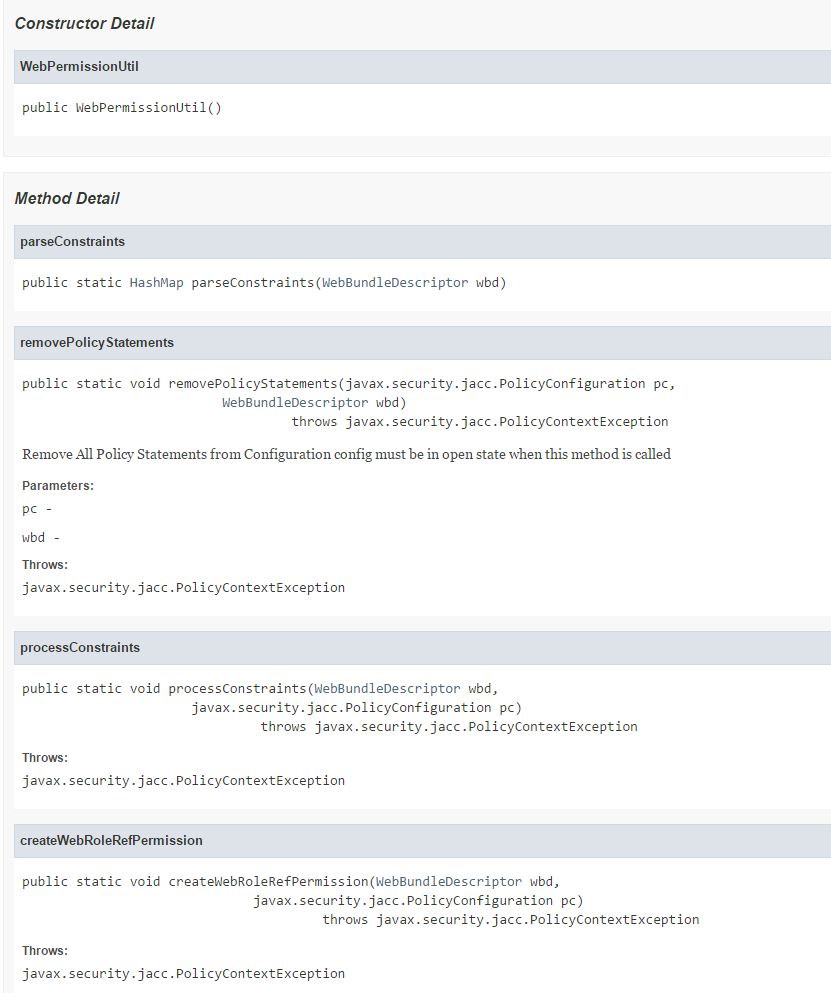
\includegraphics[keepaspectratio=true,scale=0.5]{Pictures/Javadoc}}
				\end{minipage} \linebreak
		\end{enumerate}
		
%		\subsection*{Package and Import Statements}\begin{enumerate}[resume]
%			\item If any package statements are needed, they should be the first non-comment statements. Import statements follow.
%		\end{enumerate}
		
		\pagebreak
		\subsection*{Class and Interface Declarations}\begin{enumerate}[resume]
			\setcounter{enumi}{24}
			\item \textbf{The class or interface declarations shall be in the following order:}
			\begin{enumerate}
				\item class/interface documentation comment;
				\item class or interface statement;
				\item class/interface implementation comment, if necessary;
				\item class (static) variables;
				\begin{enumerate}
					\item first public class variables;
					\item next protected class variables;
					\item next package level (no access modifier);
					\item last private class variables.
				\end{enumerate}
				\item instance variables;
				\begin{enumerate}
					\item first public instance variables;
					\item next protected instance variables;
					\item next package level (no access modifier);
					\item last private instance variables.
				\end{enumerate}
				\item constructors;
				\item methods.
			\end{enumerate}\smallskip
				At line 69, the class constructor is before the list of private static variables, as shown below.
				\lstinputlisting[title=abstract from method ``processConstraints'',numbers=left,firstnumber=65,firstline=65,lastline=76,language=Java,frame=single,breaklines=true,backgroundcolor=\color{aliceblue},basicstyle=\footnotesize,xleftmargin=17pt,showstringspaces=false,tabsize=4]{"Code/WebPermissionUtil.java"}
			\item \textbf{Methods are grouped by functionality rather than by scope or accessibility.}\smallskip \\
				Methods are grouped by accessibility rather than by functionality; in order there are package level methods, public methods and finally private methods.
%			\item Check that the code is free of duplicates, long methods, big classes, breaking encapsulation, as well as if coupling and cohesion are adequate.
			\setcounter{enumi}{27}
		\end{enumerate}
		\pagebreak
		
		\subsection*{Initialization and Declarations}\begin{enumerate}[resume]
%			\item Check that variables and class members are of the correct type. Check that they have the right visibility (public/private/protected).
			\setcounter{enumi}{28}
%			\item Check that variables are declared in the proper scope.
			\setcounter{enumi}{29}
			\item \textbf{Check that constructors are called when a new object is desired.}\smallskip \\
				The following example represents a case in which the declaration (line 494) may be split in declaration and assignment.
				\lstinputlisting[title=abstract from method ``processConstraints'',numbers=left,firstnumber=494,firstline=494,lastline=497,language=Java,frame=single,breaklines=true,backgroundcolor=\color{aliceblue},basicstyle=\small,xleftmargin=17pt,showstringspaces=false,tabsize=4]{"Code/WebPermissionUtil.java"}
				The same is for lines: 382, 384, 413, 438, 510, 541, 548, 560, 566.\\
				Moreover at line 404 the constructor is not called before the assignment done at line 415.
				\lstinputlisting[title=abstract from method ``handleConnections'',numbers=left,firstnumber=402,firstline=402,lastline=416,language=Java,frame=single,breaklines=true,backgroundcolor=\color{aliceblue},basicstyle=\small,xleftmargin=17pt,showstringspaces=false,tabsize=4]{"Code/WebPermissionUtil.java"}
%			\item Check that all object references are initialized before use.
%			\item Variables are initialized where they are declared, unless dependent upon a computation.
			\pagebreak
			\setcounter{enumi}{32}
			\item \textbf{Declarations appear at the beginning of blocks (A block is any code surrounded by curly braces `\texttt{\{}' and `\texttt{\}}'). The exception is a variable can be declared in a \texttt{for} loop.} \smallskip \\
				In the following example the \texttt{if} statement at line 488 must be postponed till after line 501 and line 508 must be put before the block of line 502.
				\lstinputlisting[title=abstract from method ``processConstraints'',numbers=left,firstnumber=484,firstline=484,lastline=508,language=Java,frame=single,breaklines=true,backgroundcolor=\color{aliceblue},basicstyle=\small,xleftmargin=17pt,showstringspaces=false,tabsize=4]{"Code/WebPermissionUtil.java"}
				The same is for:
				\begin{itemize}
					\item line 451 should occur at line 412
					\item line 539 must be before line 537
					\item line 564 must be before line 561
					\item lines 662 and 663 must be before line 657
				\end{itemize}
		\end{enumerate}
		
%		\subsection*{Method Calls}\begin{enumerate}[resume]
%			\item Check that parameters are presented in the correct order.
%			\item Check that the correct method is being called, or should it be a different method with a similar name.
%			\item Check that method returned values are used properly.
%		\end{enumerate}
%		
%		\subsection*{Arrays}\begin{enumerate}[resume]
%			\item Check that there are no off-by-one errors in array indexing (that is, all required array elements are correctly accessed through the index).
%			\item Check that all array (or other collection) indexes have been prevented from going out-of-bounds.
%			\item Check that constructors are called when a new array item is desired.
%		\end{enumerate}
		
%		\subsection*{Object Comparison}\begin{enumerate}[resume]
%			\setcounter{enumi}{39}
%			\item Check that all objects (including Strings) are compared with \texttt{equals} and not with \texttt{==}.
%		\end{enumerate}
		
%		\subsection*{Output Format}\begin{enumerate}[resume]
%			\item Check that displayed output is free of spelling and grammatical errors.
%			\item Check that error messages are comprehensive and provide guidance as to how to correct the problem.
%			\item Check that the output is formatted correctly in terms of line stepping and spacing.
%		\end{enumerate}
		
		\subsection*{Computation, Comparisons and Assignments}\begin{enumerate}[resume]
%			\item Check that the implementation avoids ``brutish programming'': (see \url{http://users.csc.calpoly.edu/~jdalbey/SWE/CodeSmells/bonehead.html}). 
%			\item Check order of computation/evaluation, operator precedence and parenthesizing.
			\setcounter{enumi}{45}
			\item \textbf{Check the liberal use of parenthesis is used to avoid operator precedence problems.}\smallskip \\
				At line 637 some parentheses could be used as in the first part of the line.
				\lstinputlisting[title=abstract from method ``createWebRoleRefPermission'',numbers=left,firstnumber=637,firstline=637,lastline=638,language=Java,frame=single,breaklines=true,backgroundcolor=\color{aliceblue},basicstyle=\small,xleftmargin=17pt,showstringspaces=false,tabsize=4]{"Code/WebPermissionUtil.java"}
%			\item Check that all denominators of a division are prevented from being zero.
%			\item Check that integer arithmetic, especially division, are used appropriately to avoid causing unexpected truncation/rounding.
%			\item Check that the comparison and Boolean operators are correct.
%			\item Check throw-catch expressions, and check that the error condition is actually legitimate.
%			\item Check that the code is free of any implicit type conversions.
		\end{enumerate}
		
%		\subsection*{Exceptions}\begin{enumerate}[resume]
%			\item Check that the relevant exceptions are caught.
%			\item Check that the appropriate action are taken for each catch block.
%		\end{enumerate}
%		
%		\subsection*{Flow of Control}\begin{enumerate}[resume]
%			\item In a \texttt{switch} statement, check that all cases are addressed by break or return.
%			\item Check that all switch statements have a default branch.
%			\item Check that all loops are correctly formed, with the appropriate initialization, increment and termination expressions.
%		\end{enumerate}
%		
%		\subsection*{Files}\begin{enumerate}[resume]
%			\item Check that all files are properly declared and opened.
%			\item Check that all files are closed properly, even in the case of an error.
%			\item Check that EOF conditions are detected and handled correctly.
%			\item Check that all file exceptions are caught and dealt with accordingly.
%		\end{enumerate}
%		
%	
%	\section{Any other problem you have highlighted}
	

	\section{Appendix}
	
	\subsection{Software and tools used}
		\begin{itemize}
			\item TeXstudio 2.10.4 (\href{http://www.texstudio.org/}{http://www.texstudio.org/}) to redact and format this document.
			\item NetBeans 8.1 (\href{https://netbeans.org/}{https://netbeans.org/}) to download and inspect the code.
			\item Sublime Text (\href{http://www.sublimetext.com/}{http://www.sublimetext.com/}) to inspect the code.
		\end{itemize}
		
	\subsection{Hours of work} The time spent to redact this document:
		\begin{itemize}
			\item Baldassari Alessandro: 20 hours.
			\item Bendin Alberto: 20 hours.
			\item Giarola Francesco: 20 hours.
		\end{itemize}
\end{document}